\documentclass[11pt]{article}

\usepackage{url}
\usepackage{hyperref}
\usepackage{graphicx}
\setlength{\parskip}{0.5cm plus4mm minus3mm}

\textwidth=6.4in
\textheight=8.5in
\hoffset=-0.7in
\voffset=-0.7in

\setlength{\parindent}{0cm} 

\newcommand{\Yfun}{Y}

\hyphenation{Text-Wrangler}

\title{Choice of geophone layout in a simple near-surface seismics setting}
\date{\today}
\author{Alain Plattner}

\begin{document}
\maketitle

\section{Introduction}
When running a near-surface seismic survey, the resulting recorded
wave forms will consist of overlapping arrivals from air waves, direct
waves, reflected waves, and refracted waves. Correctly identifying
these waves and picking their onsets, in particular of the direct and
refracted waves, is crucial for refraction and reflection seismics.

The waveforms recorded by the geophones always contain
superimpositions of the different types of seismic waves which can
make their identification difficult.  The only parameter we can
control is the layout of the geophones. See Fig.~\ref{seismicwaves}
for a sketch of the geometry.

In many settings we do have a basic idea of the depth of an interface
and rough estimations for the seismic velocities of the direct
subsurface and the underlying layer.  In this activity we use this
information to simulate arrival times and recorded waveforms. We then
vary the geophone spacing (assuming a fixed number of available
geophones and the shot at the center) to obtain an ideal setting to
identify the arrival times of specific waves.


\begin{figure}
  \center
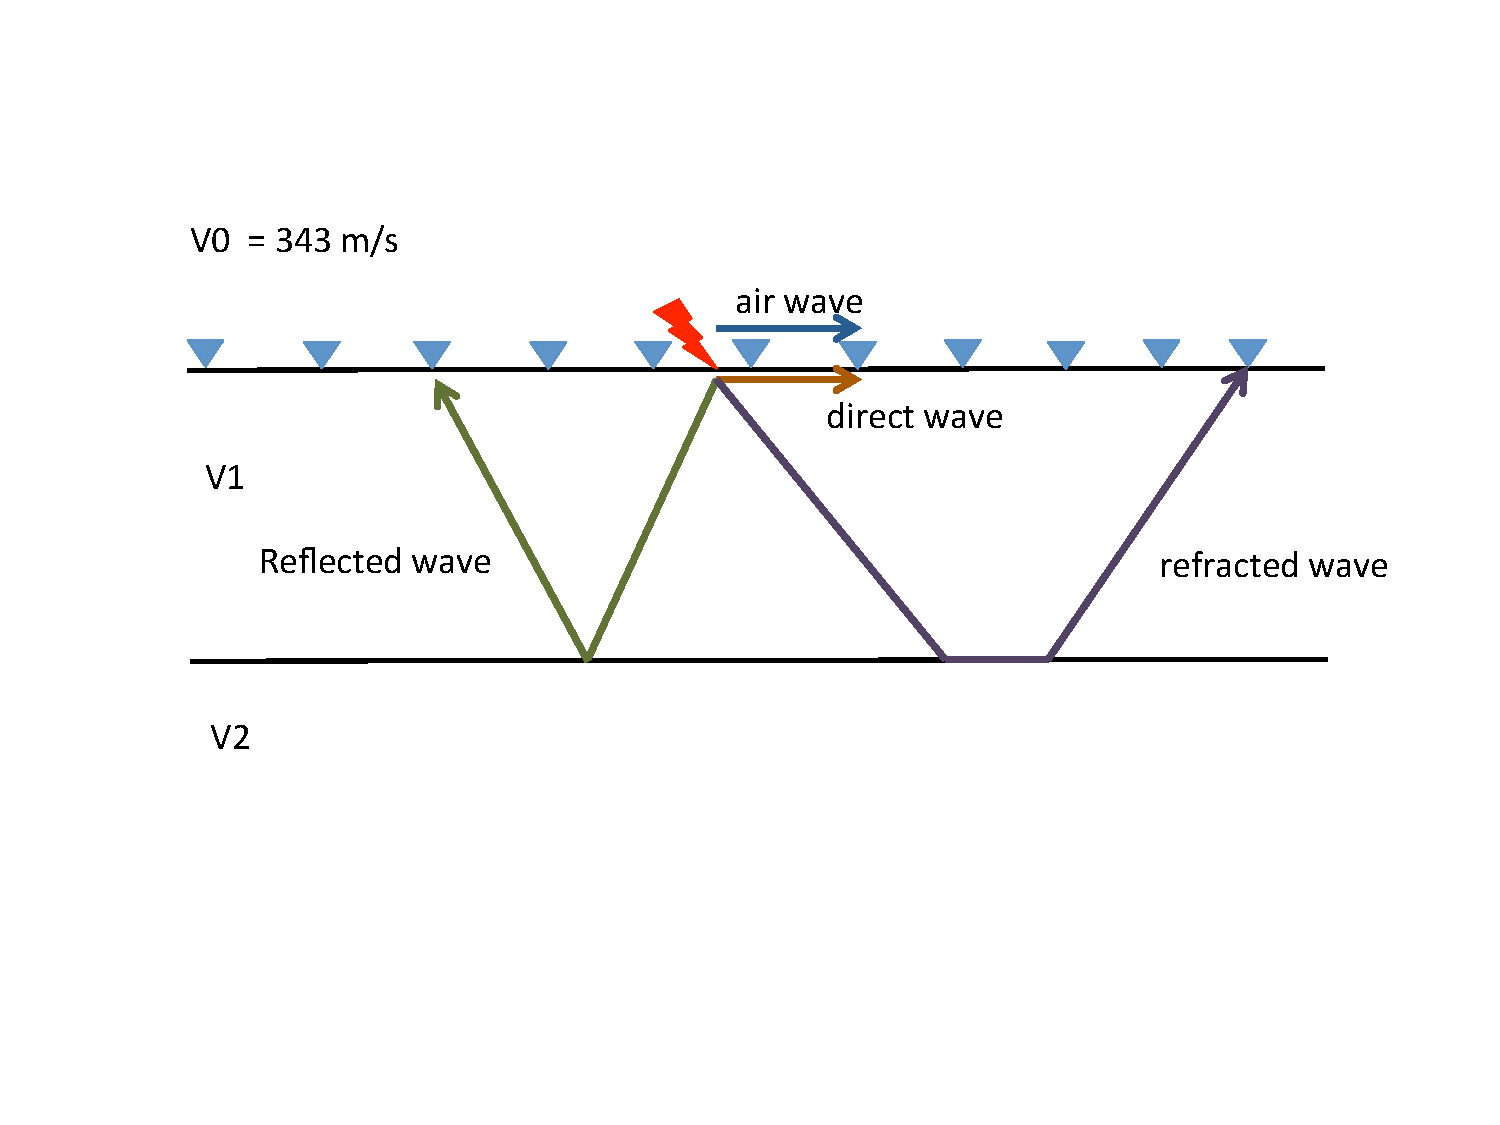
\includegraphics[width=0.7\textwidth, trim = 3cm 6cm 1.5cm
  3.5cm,clip]{figures/NSSeismics.pdf}
\caption{\label{seismicwaves} Air wave, direct wave, reflected wave,
  and refracted wave in a near-surface seismics setting. The flash
  represents the seismic source, the triangles are the geophones.}
\end{figure}

\section{Required \textsc{Matlab}/\textsc{Octave} functions}
All the \textsc{Matlab}/\textsc{Octave} functions needed for this activity can be
downloaded from the Seism-O GitHub repository

\url{https://github.com/NSGeophysics/Seism-O}

You can directly download the entire repository using Git
(\url{https://git-scm.com/}) by running in a command window

\verb#git clone https://github.com/NSGeophysics/Seism-O.git#

\section{Simulation of arrival times}
Let's assume that in this setting we have a horizontal interface at
depth \verb#h# = 2 m with shallow seismic velocity \verb#V1# = 600 m/s
and deeper seismic velocity \verb#V2# = 1000 m/s. Let's start with
setting the geophone offset (distance between geophones) to
\verb#offset# = 1 m.

After you start \textsc{Matlab}/\textsc{Octave} , switch to the folder in which you
installed the Seism-O \textsc{Matlab}/\textsc{Octave}  functions. In \textsc{Matlab}/\textsc{Octave},
run

\verb#>> [x1,t1]=showReflectedWave(V1,offset,h);#

The resulting figure (Fig.~\ref{arrivalreflect}) shows the arrival
times of the reflected wave.

\begin{figure}
  \centering
  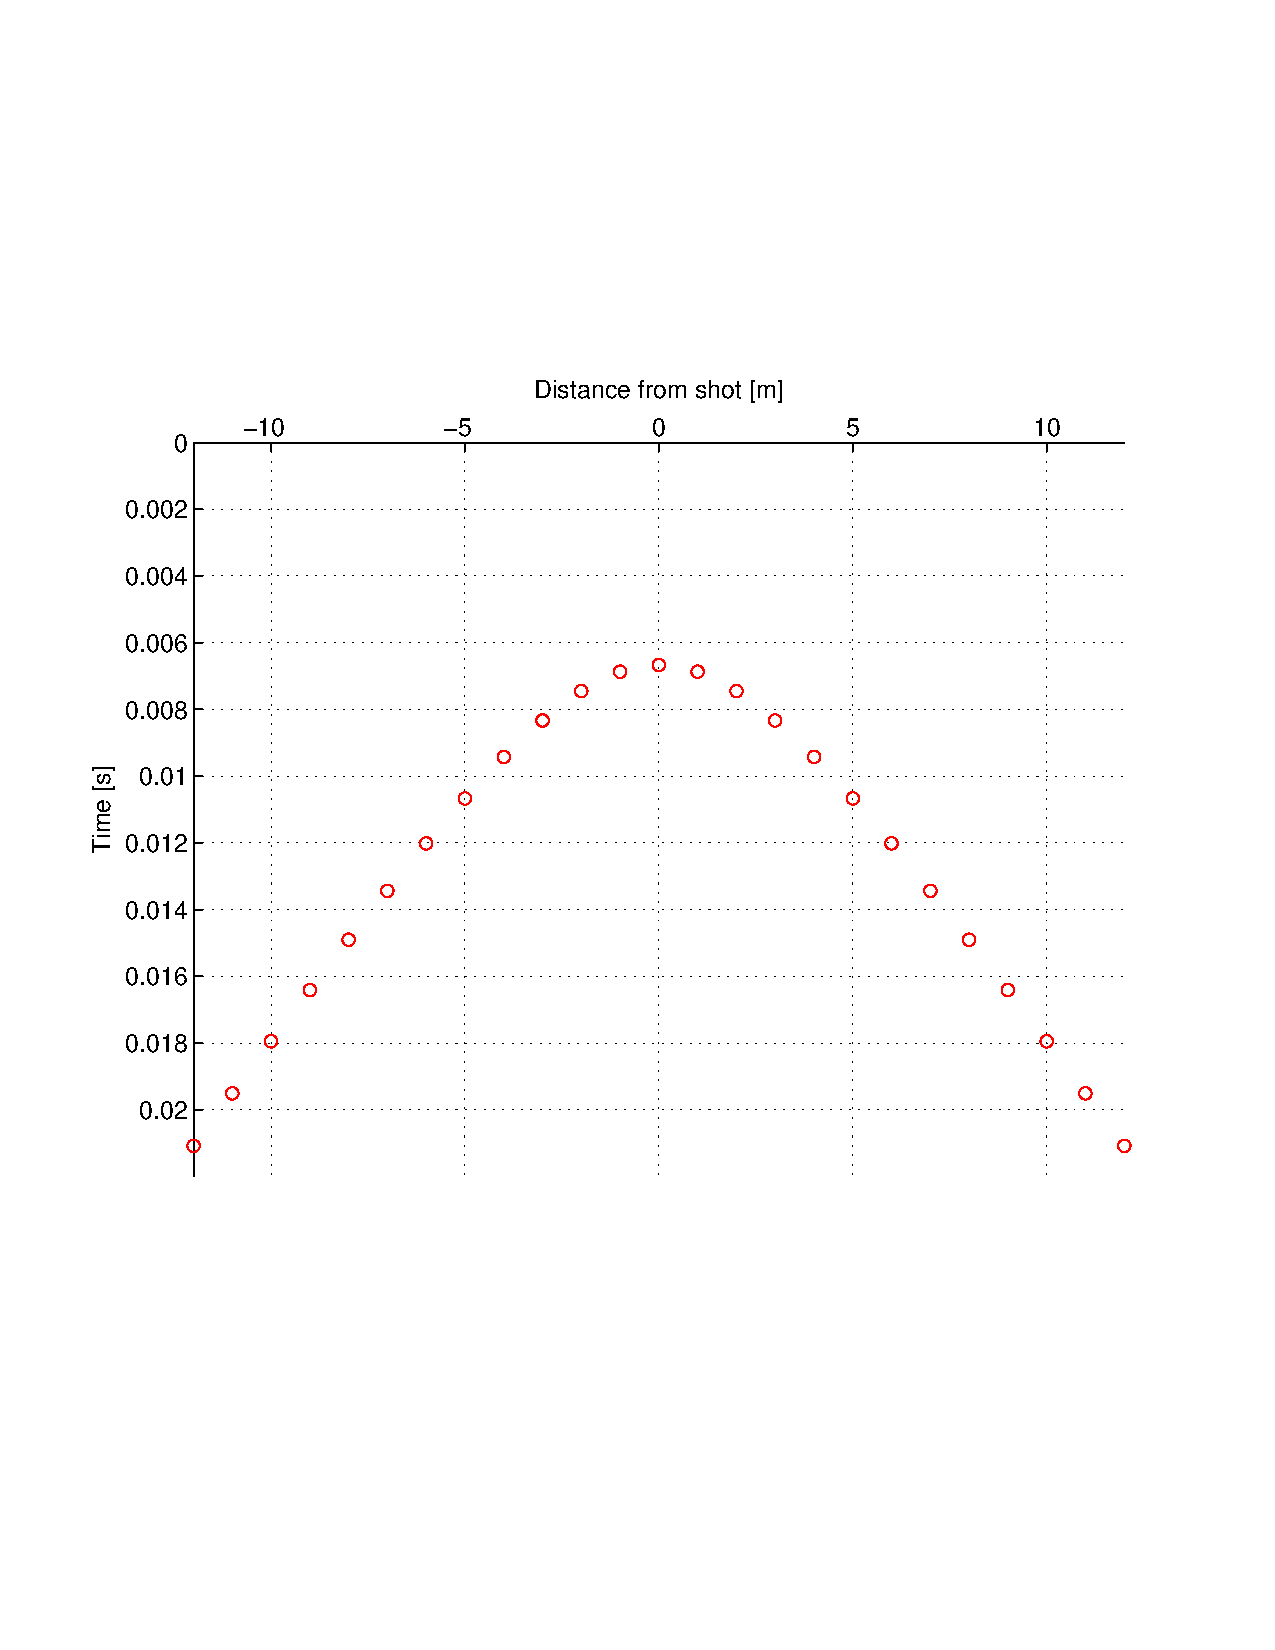
\includegraphics[width=0.7\textwidth, trim = 1cm 7.5cm 2cm
    6cm,clip]{figures/ArrivalReflected.pdf}
  \caption{\label{arrivalreflect} Arrival times of the reflected
    wave with wave velocity 600 m/s, reflector depth 2 m and geophone
    spacing 1 m.}
\end{figure}

\section{Simulation of recorded waveforms}

To show how the corresponding recorded waveforms look like, run

\verb#>> figure#\\
\verb#>> shotgather(x1,t1);#

The resulting figure should look like Fig.~\ref{reflectwave}.

\begin{figure}
  \centering
  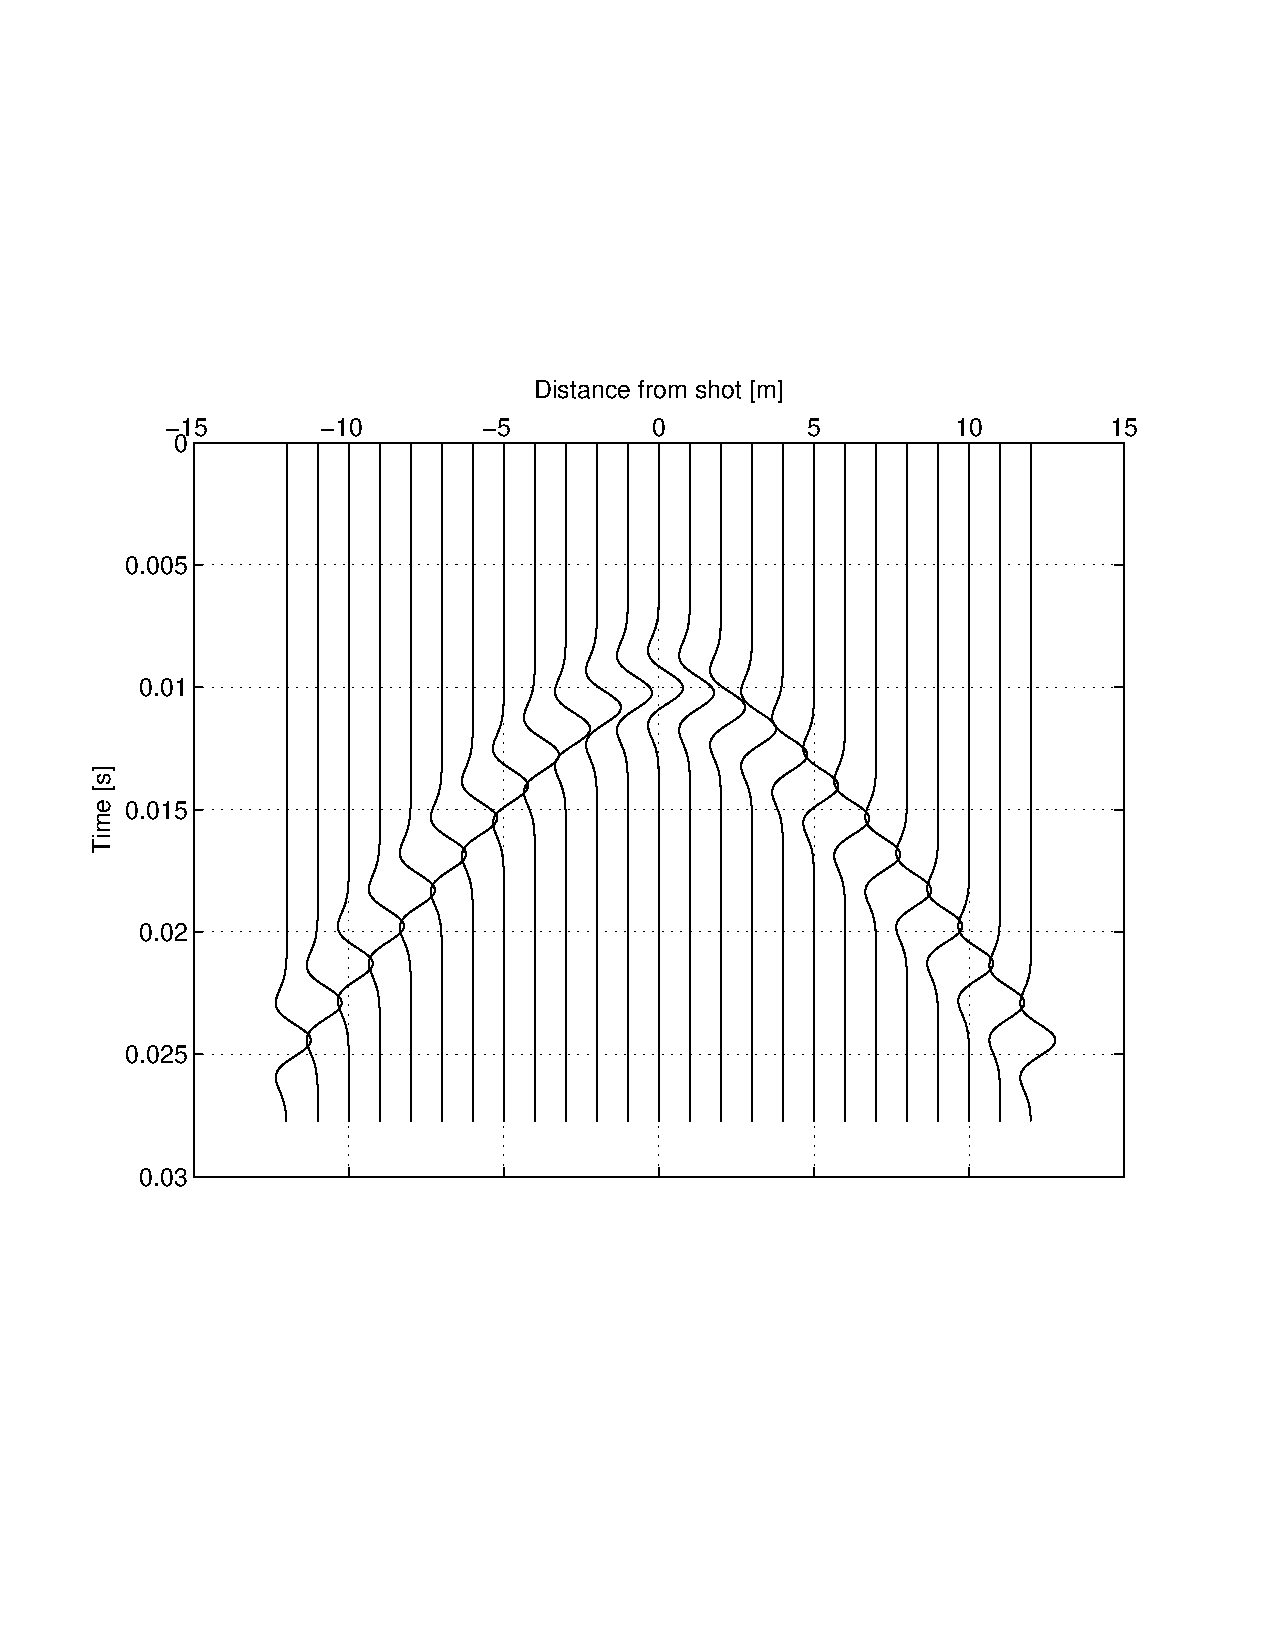
\includegraphics[width=0.7\textwidth, trim = 1cm 7.5cm 2cm
    6cm,clip]{figures/ReflectedWave.pdf}
  \caption{\label{reflectwave} Recorded waveforms (shotgather) of the
    reflected wave with wave velocity 600 m/s, reflector depth 2 m and
    geophone spacing 1 m.}
\end{figure}

\section{Superimposed waveforms}

Let's see how a direct wave plotted together with a reflected wave
would look like. To see how the picked arrival times overlap, run

\verb#>> figure(1)#\\
\verb#>> [x2,t2]=showDirectWave(V1,offset);#

For geophones away from the source, the arrival times of the direct
and the reflected wave will be close together. The identification gets
more difficult when looking at the shot gather:

\verb#>> seis1=shotgather(x1,t1);#\\
\verb#>> seis2=shotgather(x2,t2);#\\
\verb#>> seis=addgather(seis1,seis2);#\\
\verb#>> figure#\\
\verb#>> plotgather(seis)#

The result should look like Fig.~\ref{directreflect}.

\begin{figure}
  \centering
  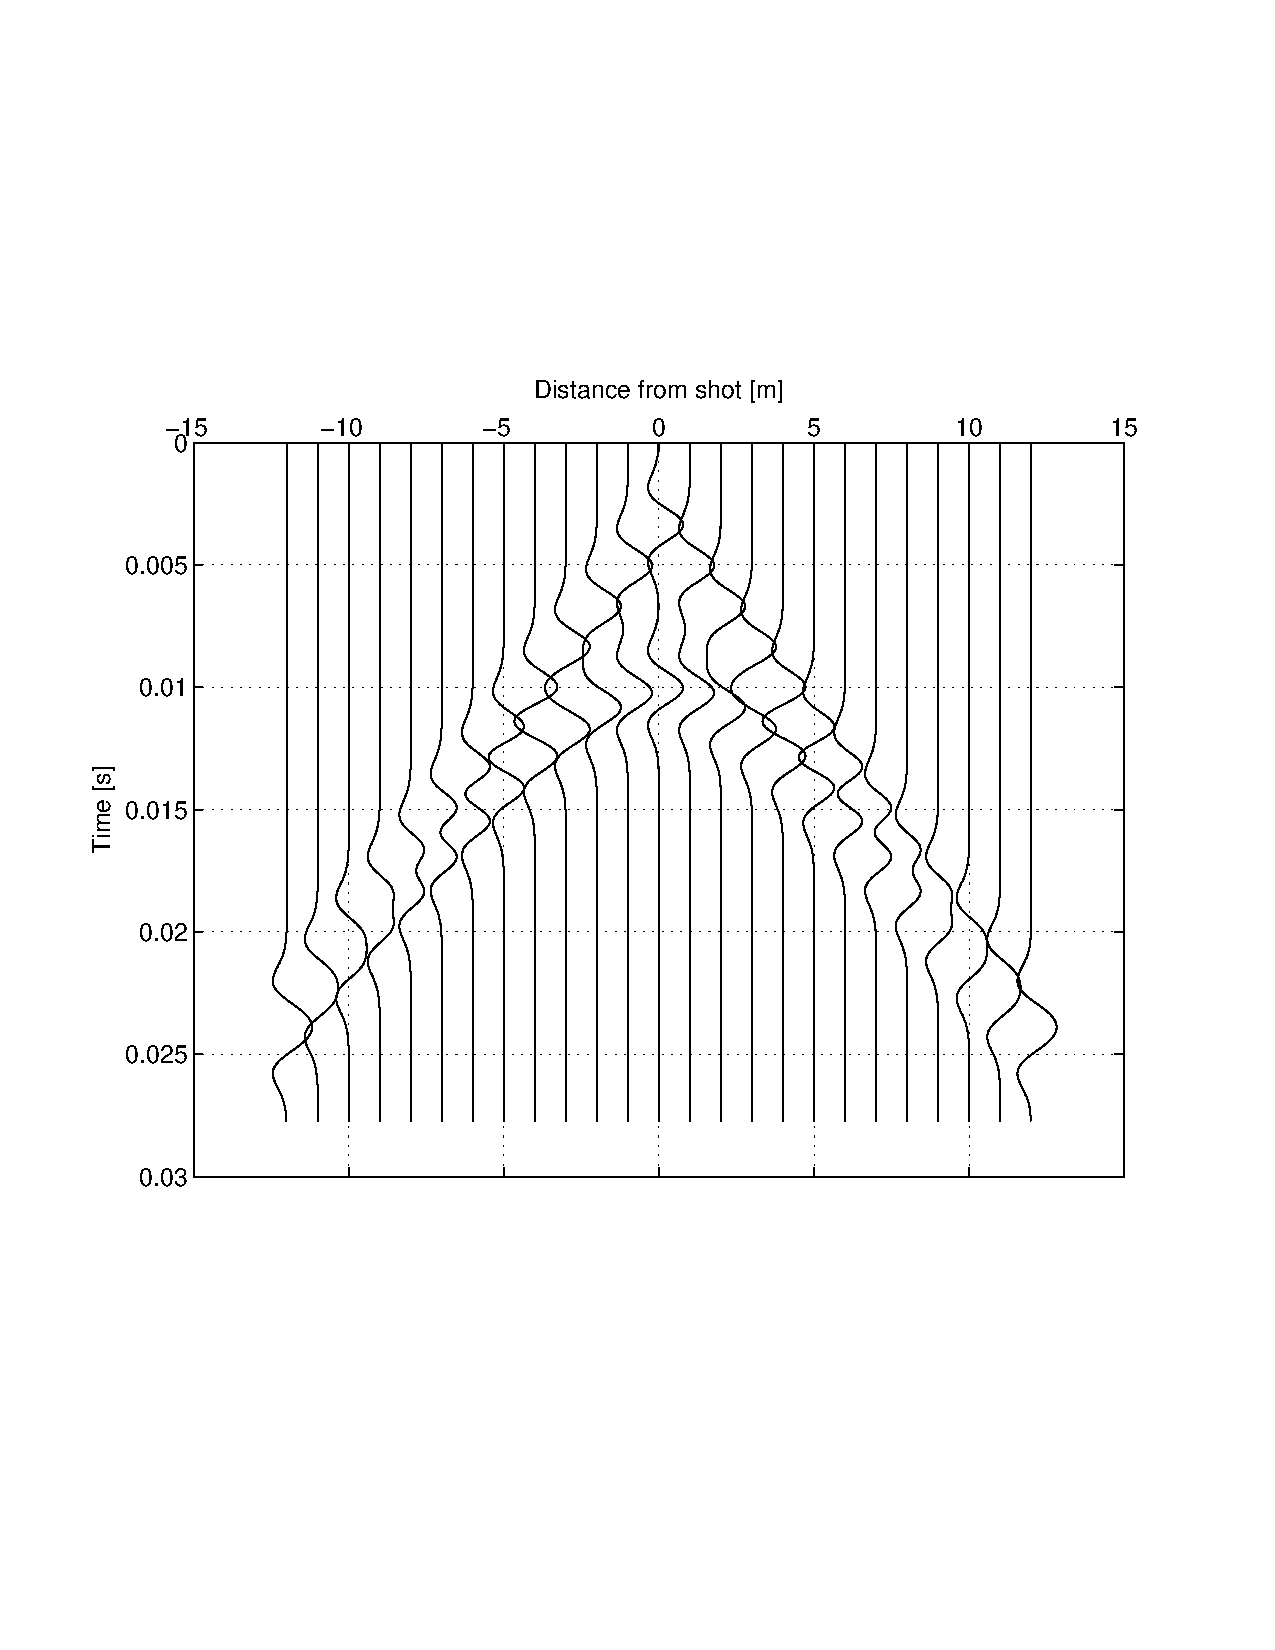
\includegraphics[width=0.7\textwidth, trim = 1cm 7.5cm 2cm
    6cm,clip]{figures/DirectReflected.pdf}
    \caption{\label{directreflect} Recorded waveforms (shotgather) of
      the reflected wave and direct wave superimposed. Wave
      velocity is 600 m/s, reflector depth is 2 m and geophone spacing
      is 1 m.}
\end{figure}

Finally, the \textsc{Matlab}/\textsc{Octave} function \verb#showAllWaves.m#
superimposes the waveforms of the air wave, the direct wave, the
reflected wave, and a refracted wave:

\verb#>> seis=showAllWaves(V1,offset,h,V2);#\\
\verb#>> figure#\\
\verb#>> plotgather(seis);#

The resulting superimposed waveforms (Fig.~\ref{allwaves}) are
difficult to discern.

\begin{figure}
  \centering
  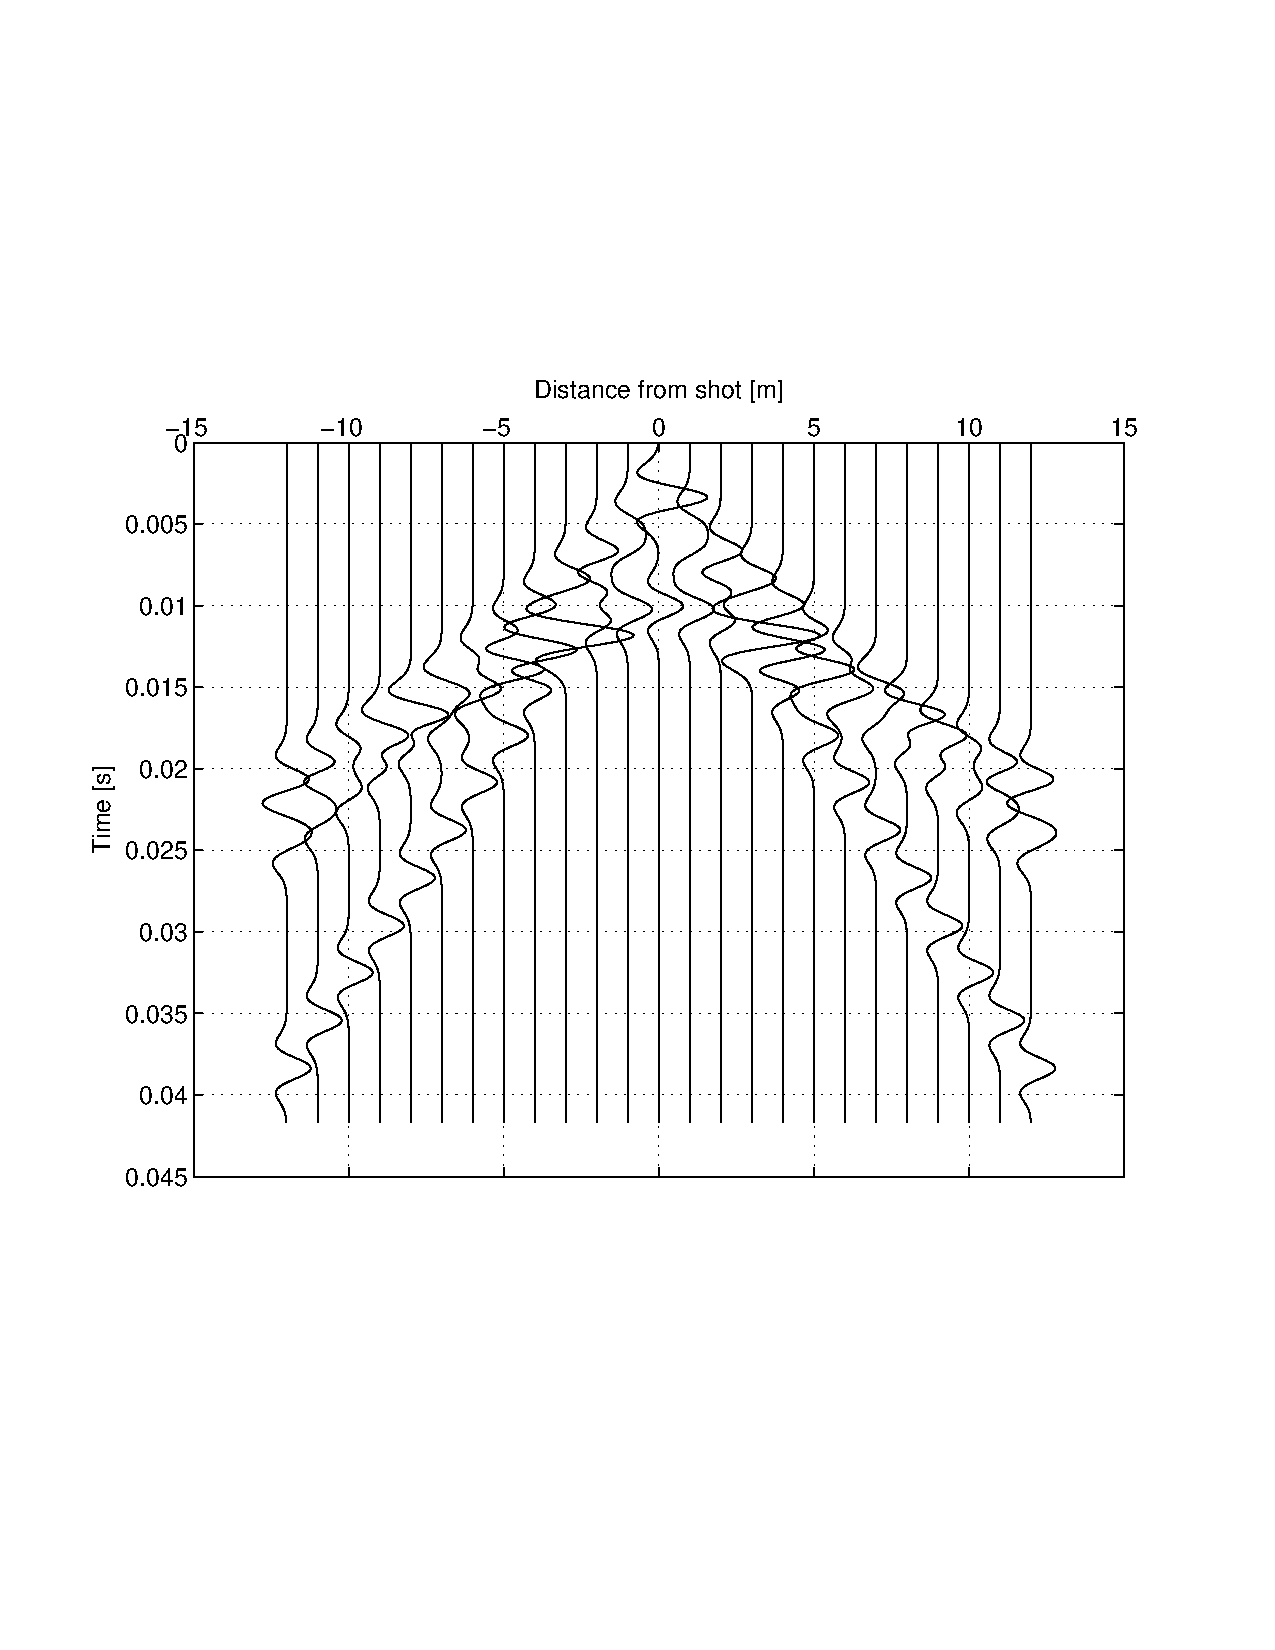
\includegraphics[width=0.7\textwidth, trim = 1cm 7.5cm 2cm
    6cm,clip]{figures/AllWaves.pdf}
  \caption{\label{allwaves} Recorded waveforms (shotgather) of the air
    wave, direct wave, reflected wave, and refracted wave
    superimposed. Shallow wave velocity is 600 m/s, deep wave velocity
    is 1000 m/s, reflector depth is 2 m and geophone spacing is 1
    m. It is difficult to tell the refracted, reflected, and direct
    waves apart. The air wave stands out as the slowest wave and can
    at distances greater than 7 m be identified.}
\end{figure}

\section{Choosing the right geophone layout}

Remember that the only parameter we can choose in a such a setting is
the geophone layout (spacing, if we only have a fixed number of
geophones).

\textbf{Exercise:} Play with the geophone spacing and find a value
that allows us to easily identify the refracted wave.

\textbf{Exercise:} Choose a different setting, for example \verb#V1# =
600 m/s, \verb#V2# = 2000 m/s, \verb#h# = 10 m. Find a suited geophone
spacing value for this situation.

Explore the rest of the Seism-O package. For example, it allows to
plot common depth point gathers and attempt a (simplified) normal
move-out correction.


\end{document}
